\documentclass[12pt,a4paper,twoside]{article}

\usepackage[english]{babel}

%------------------------------ encoding
\usepackage[utf8]{inputenc}
\usepackage{csquotes}

%------------------------------ page layout
\usepackage[left=3cm,right=3cm,top=3cm,bottom=2cm]{geometry}

%------------------------------ clickable toc and links styles
\usepackage{hyperref}
\hypersetup{
    colorlinks,
    citecolor=black,
    filecolor=black,
    linkcolor=black,
    urlcolor=black
}

%------------------------------ font macro
\newcommand*{\courierfont}{\fontfamily{pcr}\selectfont}

%------------------------------ references
\usepackage{biblatex}
\addbibresource{bib.bib}

%------------------------------ tables
\usepackage{tabularx}

%------------------------------ images
\usepackage{graphicx}
\usepackage{subcaption}

%------------------------------ font preferences (1) or sc
\usepackage[sc]{mathpazo} 
% \usepackage{newpxmath}

%------------------------------ comment
\usepackage{comment}

%------------------------------ title spec
\usepackage{titlesec}
\usepackage{afterpage}

%------------------------------ abstract
\usepackage{abstract}
\renewcommand{\abstractnamefont}{\normalfont\Large\bfseries}

%------------------------------ page numbering
\usepackage{lastpage}
\usepackage{fancyhdr}
\pagestyle{fancy}
\fancyhf{}
\fancyfoot[R]{\thepage \hspace{1pt} of \pageref{LastPage}}

\begin{document}

\begin{comment}
\begin{titlepage}
    \centering
    \vspace*{\fill}

    \vspace*{0.5cm}
    
    \huge ACULEI
    
    \vspace*{2.5cm}
    
    \vspace*{1cm}

    \begin{minipage}{\textwidth}
        \centering
        \begin{tabular}{ccc}
            \small \textbf{Brajucha Filippo} & \small \textbf{Dinelli Michele} & \\
            \small University of Bologna & \small University of Bologna & \\
            \scriptsize \courierfont{\href{mailto:filippo.brajucha@studio.unibo.it}{filippo.brajucha@studio.unibo.it}} & \scriptsize \courierfont{\href{mailto:michele.dinelli5@studio.unibo.it}{michele.dinelli5@studio.unibo.it}} & \\
        \end{tabular}
    \end{minipage}

    \vspace*{1cm}

    \begin{minipage}{\textwidth}
        \centering
        \begin{tabular}{ccc}
            \small \textbf{Hanna Youssef} \\
            \small University of Bologna \\
            \scriptsize \courierfont{\href{mailto:youssefawni.hanna@studio.unibo.it}{youssefawni.hanna@studio.unibo.it}} \\
        \end{tabular}
    \end{minipage}
    
    \vspace*{\fill}
\end{titlepage}

\tableofcontents

\newpage

\end{comment}

\begin{center}

\rule[0.1cm]{15.8cm}{1.5mm}
{{\Large{Aculei}}} 
\rule[0.1cm]{15.8cm}{0.1mm}

\vspace*{1cm}

\begin{minipage}{\textwidth}
    \begin{tabular}{ccc}
        \small \textbf{Brajucha Filippo} & \small \textbf{Dinelli Michele} & \small \textbf{Hanna Youssef} \\
        \small University of Bologna & \small University of Bologna & \small University of Bologna \\
        \scriptsize \texttt{\href{mailto:filippo.brajucha@studio.unibo.it}{filippo.brajucha@studio.unibo.it}} & \scriptsize \texttt{\href{mailto:michele.dinelli5@studio.unibo.it}{michele.dinelli5@studio.unibo.it}} & \scriptsize \texttt{\href{mailto:youssefawni.hanna@studio.unibo.it}{youssefawni.hanna@studio.unibo.it}} \\
    \end{tabular}
\end{minipage}

\vspace*{1cm}
    
\end{center}

\begin{abstract}    
\noindent This report describes the steps in the process of building a dataset that collects data from photographs of animals taken automatically by photo-traps located in the forests of Umbria. Realizing the dataset aims to collect a vast amount of data, so as to put it at the service of artificial intelligence techniques in order to group and potentially classify the photographs. \\ Two approaches are explored: the first involves unsupervised learning based on algorithms of clustering, while the second is based on a technique called \textit{zero-shot image classification} in order to classify photographs according to the animal portrayed. \\ 
In recent years, the discipline known as computer vision has made enormous strides, thanks to this branch of computer science it is possible to manipulate complex data, such as photographs, extracting knowledge from them. The information obtained from photographs, the relationships and hidden patterns that are identified by artificial intelligence are used to generate an interactive experience within a photographic archive called \textit{aculei}. The project \textit{aculei} is the brainchild of a Milanese photographer who placed several automatic photo-traps in the woods surrounding the house in which he grew up in Umbria. The desire to publish the photographs and make the experience on the archive ai-driven are his motivations for conceiving the project \textit{aculei}.
\end{abstract}

\section{Introduction}
Computer vision is a field of artificial intelligence that allows computers to extract 
information and data from digital images, videos and other visual inputs. It works in much the same way as human vision, but humans have a great advantage: they have years and years of experience in which they they have trained themselves to distinguish objects \cite{ibm-comp-vision}. Computers have to do the same but in much less time by generally resorting to deeplearning techniques by exploiting a type of neural networks known as convolutional neural networks. Several techniques have been used based on computer vision such as ocr (optical character recognition) \footnote{is a term that describes the programs dedicated to optical character recognition in a document} and zero-shot image classification \footnote{a computer vision task for classifying images into a given class, without any training or prior knowledge of the classes}. \\ Computer vision was extensively exploited to realize the spines dataset since the data provided are more than 16000 digital images that must necessarily be processed by a computer.

\begin{figure}[!ht]
    \centering
    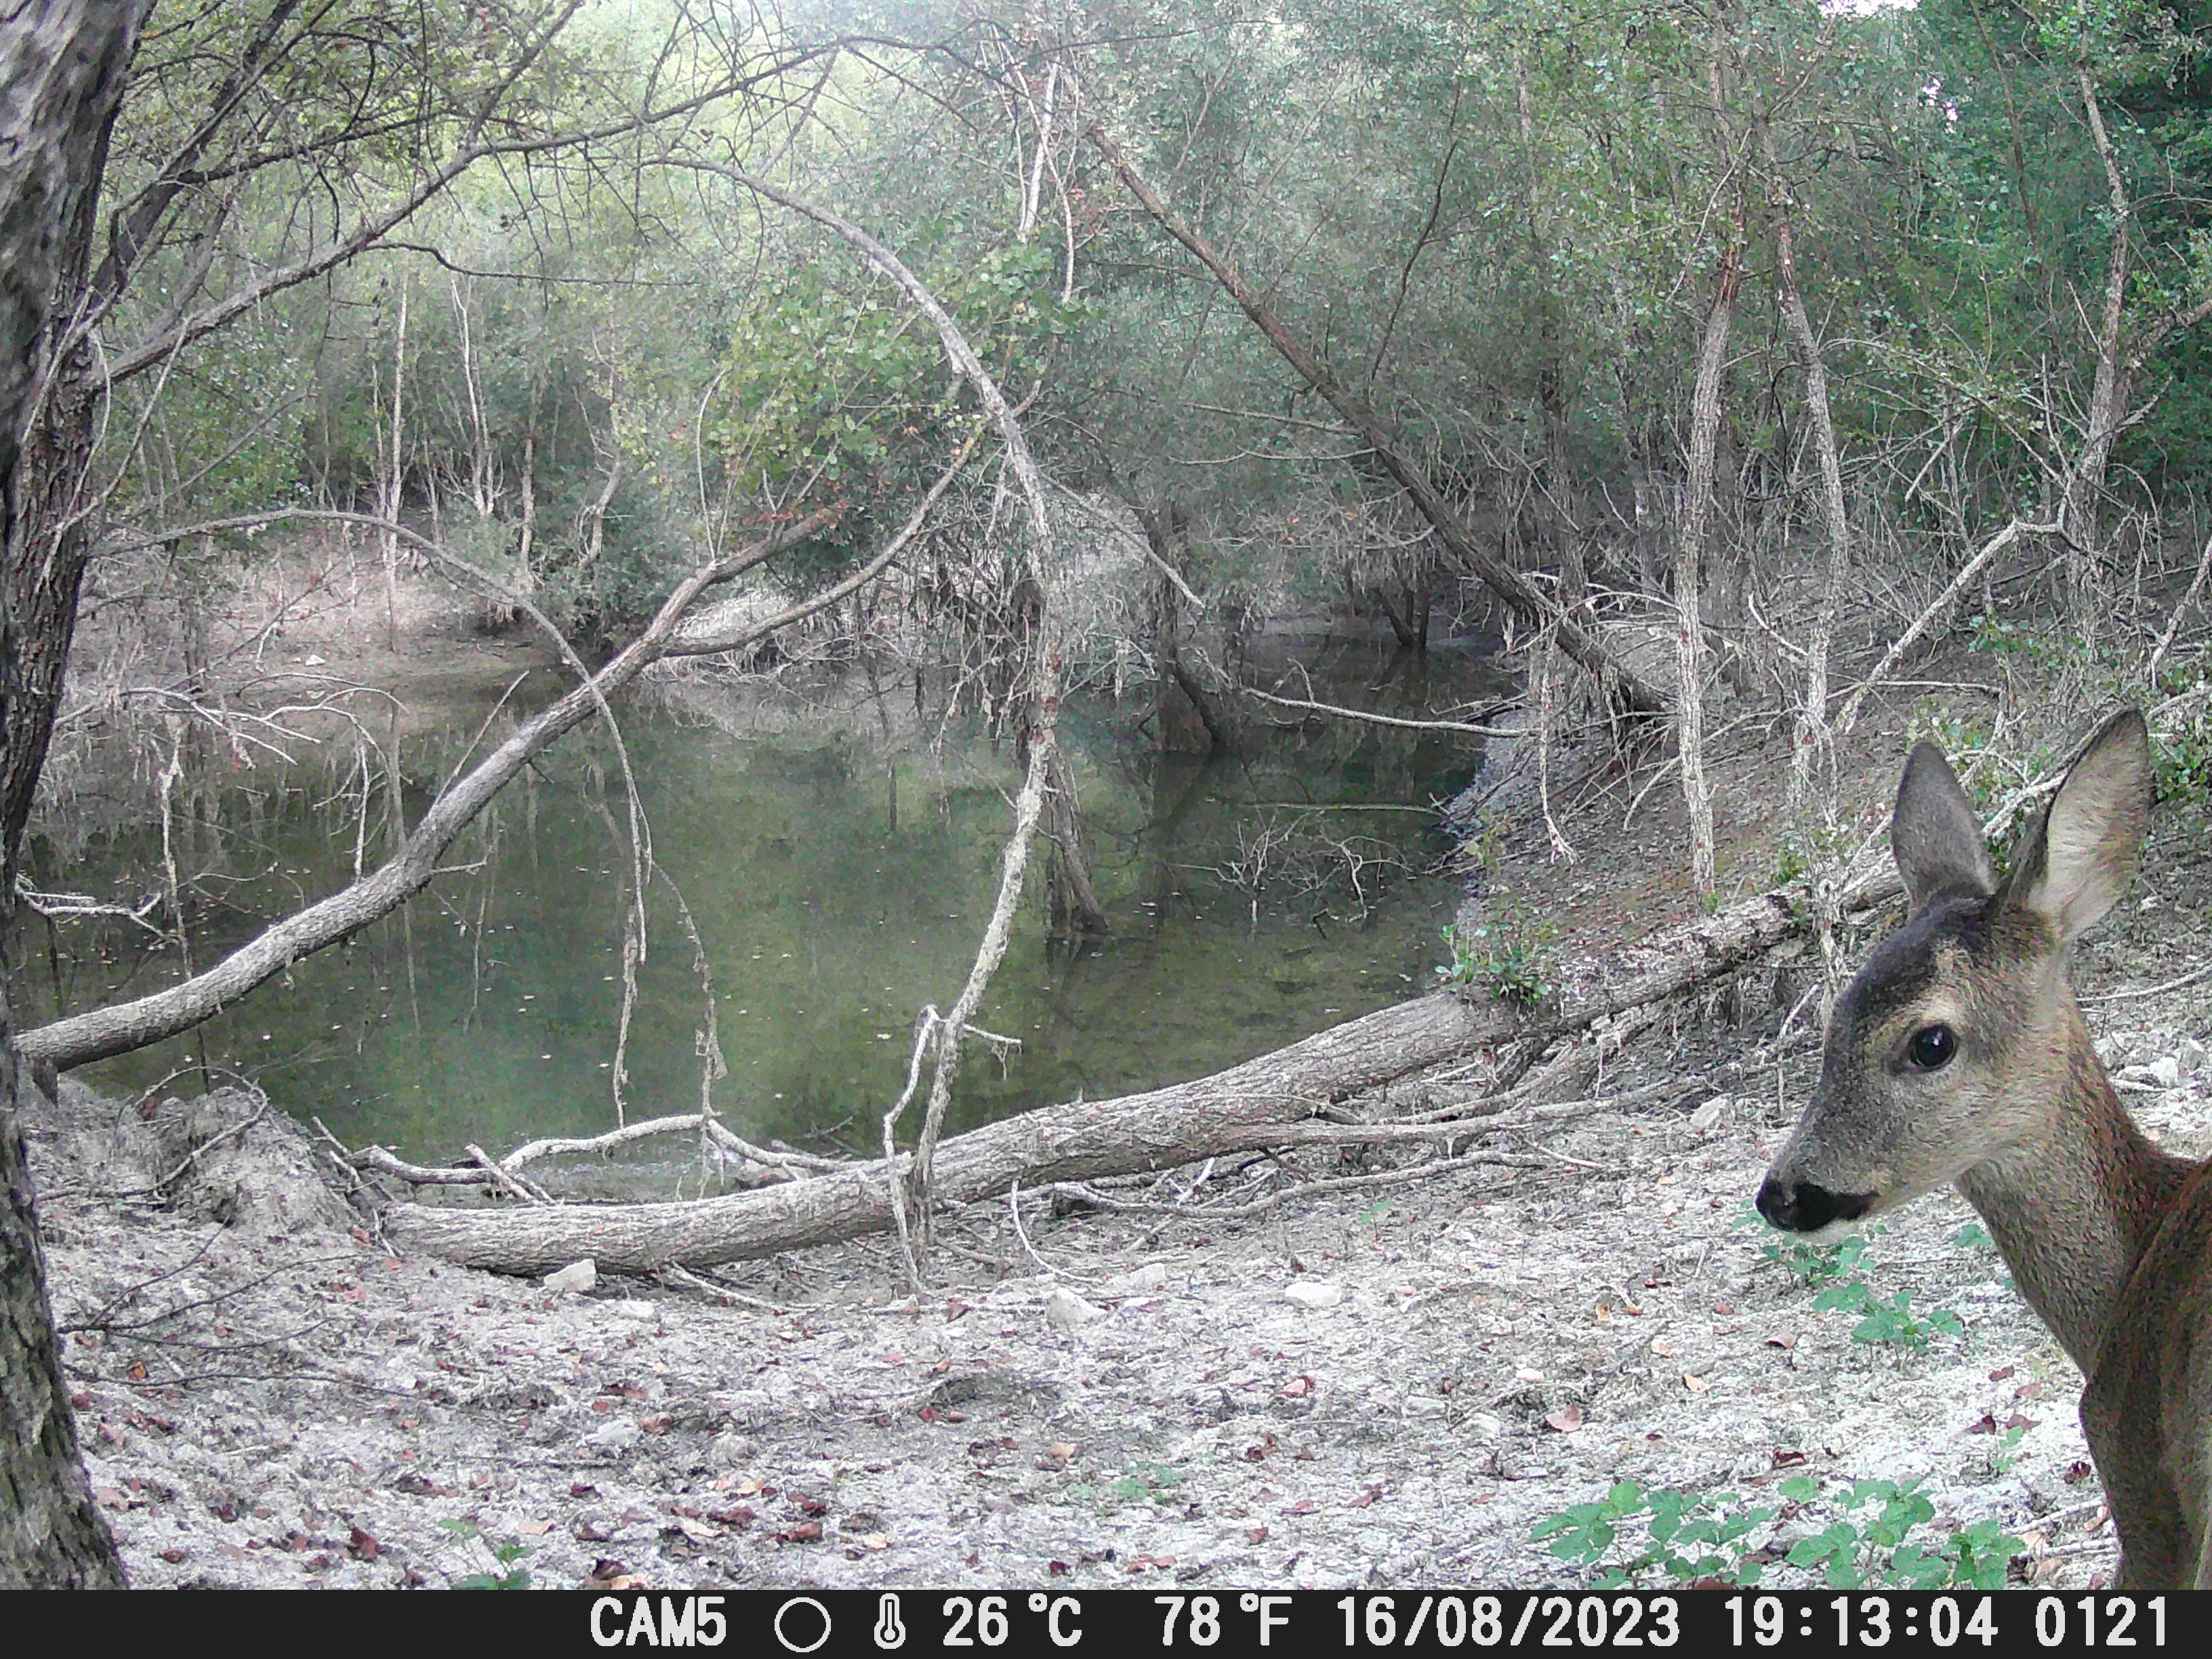
\includegraphics[width=\textwidth ,height=\textheight, keepaspectratio]{assets/TF_ACULEI_16567_DSCF0121.jpg}
    \caption{Example of a digital image taken by one of the photo-traps}
    \label{fig:TF_ACULEI_16567_DSCF0121}
\end{figure}

\subsection{Description of the problem}
You want to create a dataset containing data from photographs taken automatically from photo-traps 
placed in Umbria. The photographs were made available by the photographer owner of the 
photo-traps who has been collecting them for the past 4 years.\\
From the photographs we want to extract key data such as temperature, moon phase, the camera 
that took the image, and the date and time. Very ambitious is the recognition of the animal portrayed. Photographs may contain among the meta-data some of this information while some times it is completely absent such as temperature measurement and information on the type of 
animal. The loss of some information in the meta-data could be caused by intermediate software 
that the photographer used to process the photos before providing them for the study.\\ 
The problem then is to define a set of procedures for processing the images, extracting from them the relevant information and then create a dataset on which to apply artificial intelligence techniques to identify correlations among the photographs so as to provide an immersive experience on the archive photograph that collects them.

\subsubsection{Problem rationale and relevance}
The spines project stems from the desire of the photographer who owns the photo-traps to make public photographs. To do so, he wanted to initiate the development of an online photo archive with a strong artistic imprint. \\ In addition to studies stylistics related to interaction and user experience, a phase has been planned in which artificial intelligence is applied so that it guides the user experience on the archive. In the context of the aculei project, the phase described in this paper represents a very important point in the development of the backend system related to the photo archive.

\subsubsection{Interested audience}
People interested in this project are those who want to observe the various stages of creating 
of a dataset from data collection to the creation of the complete dataset. In addition, 
those who want to use the dataset for their own studies or expand 
and improve those at the moment carried out.

\subsubsection{Benefits of a solution}
A detailed and well-documented solution is certainly helpful in defining the steps needed to 
creation of a dataset in the most correct and meaningful way, highlighting the difficulties and strengths. \\ Making a satisfactory, orderly, and easily usable dataset also means completing the 
component that manages the interaction on the archive \textit{aculei} through the website, then 
create a platform for displaying this photographic content, making the most of its 
features. 

\subsection{Proposed Solution}

\subsubsection{Approach to the solution}
The first idea was to develop an artificial intelligence with the available images. The artificial intelligence in question would have to predict the next image to recommend to the user from the previously recommended images. The process turned out to be rather complex because of the nature of the data (high-resolution images that had to be pre-processed in a precise manner). Under the circumstances, the idea was abandoned and we focused on an unsupervised approach based on clustering algorithms. To arrive at clustering processes, however, the basis remains the creation of a dataset on which to apply unsupervised learning. \\ For the purpose of building a dataset from digital photographs, we first asked ourselves what data were present and therefore extractable from a digital photograph. As can be seen in figure \ref{fig:TF_ACULEI_16567_DSCF0121} the photographs in question have a black horizontal stripe showing some of the meta-data exported directly from the photo-trap at the time it was taken. The meta-data are: the photo-trap that took the photo (camera), moon phase, temperature, date and time. This situation introduces two problems to consider: the horizontal strip of meta-data is not always present in the photographs (for reasons not currently determined) and the meta-data are not also found in the file meta-data, they are only present in the image in the form of pixels. Given these two issues, two steps were identified in order to accurately extract meta-data from the images: meta-data reading and extraction using \textit{Exiftool} \cite{exiftool} and ocr techniques using python libraries such as \textit{PyTesseract} \cite{pytesseract} and \textit{EasyOCR} \cite{easyocr} to extractg text from images. Once the two steps were carried out, a primitive version of the dataset was obtained but rich in infromations from which knowledge could be extracted.

\subsubsection{IT challenges faced}
The main problems encountered are related to the quality of the images (which are not always optimal) and the unevenness of the data. For example, in some cases, some meta-data were successfully extracted using \textit{Exiftool}, while in other cases they were not. We had to provide fallback cases so that no information was lost. Another obstacle was time; in fact, applying OCR to photographs was not computationally fast. Some sort of pre-processing had to be provided to decrease the number of pixels that the libraries had to consult by cropping the photographs. This pre-processing added to the actual time to extract text from the images and caused several takes. We used two libraries because, comparing them, we noticed that the best results were obtained by combining and merging the two outputs. \\ Another problem faced had to do with the encoding of the dataset, which is rich in categorical variables. We had to go very deep into these terms. As well, we had to delve into how we would choose the number of clusters and how to use the dataset for unsupervised learning (PCA analysis). Another challenge faced stems from the ambition we had in wanting to extract the label of the portrayed subject from the images as well. This caused a lot of time spent, and we tried numerous approaches, evaluating various pre-designed models without fine-tuning. Finally, we agreed to the use of the zero-image classification of huggingface \cite{huggingface}.

\subsubsection{SOA: State of the art}
Zero-shot Image Classification (ZSIC) represents a cutting-edge frontier in contemporary computer vision, offering a compelling challenge and a rich domain for exploration. At its core, ZSIC involves the classification of images into distinct categories without the model's prior exposure to or explicit training on those categories. Inspired by transfer learning, the method leverages information learned from training one model to identify and categorize new classes that weren't in the original training set. \\
In addressing the complexities of ZSIC, the employed model utilizes a nuanced learning paradigm, adeptly incorporating three crucial types of data: seen data, unseen data, and auxiliary information. Seen data consists of images and corresponding labels, forming the foundational knowledge base during the model's training. In contrast, unseen data comprises solely class labels, representing uncharted territory that the model navigates and classifies. Bridging the semantic gap between these sets, auxiliary information is introduced during training, offering additional context through textual descriptions or word embeddings.\\ 
Traditionally, image classification requires training a model on a specific set of labeled images, with fine-tuning often necessary when new labels are introduced. In contrast, the approach embraces zero-shot or open vocabulary image classification, employing multi-modal models trained on extensive datasets of images and associated descriptions. These models excel at learning aligned vision-language representations, ushering in a more flexible framework for image classification. This adaptability allows the model to generalize seamlessly to new and unseen categories without additional training data, enabling users to query images using free-form text descriptions of their target objects. As we navigate the state of the art, it becomes evident that ZSIC, with its reliance on transfer learning and innovative data handling approaches, holds immense promise for reshaping the landscape of image classification, providing models with remarkable adaptability to an ever-expanding spectrum of visual concepts.

\subsubsection{Group management}
The group worked fairly evenly in the implementation of the project, all of them having 
participated in different ways in its completion. During the writing of the code, an approach in which everyone was free to criticize and advise what was the ideal solution for him. There were many situations where we got together and tried to devise and develop ideas so that we could 
solve the problems encountered along the way.

\subsubsection{Results obtained: a summary}
We obtained a dataset from photos of animals taken by photo-traps. Each row in the dataset has information at the time of the shot, such as moon phase, datetime, the most likely label of the subject pictured, a unique identifier, temperature, and season, and the photo-trap that took it. Some data is derivable but still useful for unsupervised learning tasks.

\begin{figure}[!ht]
    \centering
    \includegraphics[width=\textwidth,height=\textheight,keepaspectratio]{assets/zsic.png}
    \caption{Zero shot image classification results}
    \label{fig:}
\end{figure}

\begin{figure}[!ht]
    \centering
    \includegraphics[width=\textwidth,height=\textheight,keepaspectratio]{assets/animals-count.png}
    \caption{Zero shot image classification results considering the most probable label}
    \label{fig:}
\end{figure}

\newpage

\section{Proposed Method}
The proposed method is a dynamic process based on multiple iterations and steps, leading to the population of the dataset and subsequent clustering. This method represents a culmination of diverse approaches that were systematically tested during the execution, aiming to identify the most optimal solution for our specific requirements. In essence, we navigated through a wide array of solutions to arrive at what appeared to be the most fitting one.

\subsection{Choice of Solution}
We conducted a thorough analysis of the available dataset, comprising a substantial number of photos with information embedded in both the pixel data of the bait photos and the metadata of the images. Initially, we extracted all possible metadata using the \textit{Exiftool} \cite{exiftool} and populated the dataset.\\
Subsequently, for the results not obtained from metadata, we turned to the pixel data of the images, employing two Python tools, \textit{PyTesseract} \cite{pytesseract} and \textit{EasyOCR} \cite{easyocr}. Additional data points, such as lunar phases derived from the date, were calculated using scripts. Throughout the database population process, checks were implemented to ensure data accuracy and normalization. The outcome was a remarkably well-populated dataset. \\
Following the dataset population, the next step was to assign labels to each image representing the captured animal. To achieve this, we utilized the \textit{Hugging Face library for Zero-shot image} \cite{huggingface} classification, yielding highly positive results that facilitated individualizing each animal. \\
Ultimately, the chosen solution involved performing three types of clustering (numerical, one-hot encoded, animal-only) and analyzing the results to determine the most suitable approach for the project's final objective.

\subsubsection{Alternatives considered and justifications for the choice}
At first, the option of developing a system that could recommend an image given the previous ones was considered. This type of approach would have been possible with greater computational resources and possibly deeper machine learning techniques. It was decided to pursue unsupervised techniques (clustering) because the nature of the data was amenable to this type of learning.  

\subsubsection{Methodology for measuring performance}
Performance measurement was not trivial during development. We had to define how to evaluate the quality of the dataset we were building, and in addition we had to evaluate the results of unsupervised learning on the data. \\ To assess the quality of the dataset we performed multiple iterations refining ocr-based extraction techniques by combining them with deep reading of the meta-data. Iterating several times, we arrived at a level of liking, with the fields always present and never missing. All this except for temperature, which is a field with about 16\% missing values, often due to total missingness in the meta-data and also in the image pixels. \\ To evaluate clustering instead, we used some metrics such as silhoutte-score to assess the goodness of clusters created. Visual evaluation was also useful and was done using the photo archive showing the images according to the clustering done.

\section{Experimental Results}

\subsection{Demonstration and Technologies}

\subsubsection{Instruction for demonstration}
For a demonstration of what has been achieved you can go to the \href{https://aculei.xyz}{ACULEI} website. Alternatively, source code is provided at the end of this report that can be run by instantiating a virtual python environment and cloning the repository. Note that the images are private and are not provided within the git repository, so request them from one of the authors.\\
The result obtained by this work is a rich dataset with a lot of information gleaned from  photos.

\subsubsection{Technologies and versions}
The technologies used were python running in a notebook environment and a variety of libraries. 
The libraries used have different purposes, some are useful for the proper storage of data, others are essential for the calculation and processing of data. The versions of the libraries used can be found on the \href{https://github.com/micheledinelli/aculei-ai}{requirements.txt} file in the attached repository. 

\subsection{Results}
The end result of this attempt was a comprehensive dataset precisely created from photographs acquired by strategically positioned photo-traps. This dataset has enormous potential across multiple disciplines, acting as a solid foundation for numerous applications. It is ready to support efforts ranging from developing complex models for animal relocation projects to facilitating unsupervised learning techniques. Furthermore, its quantity of information allows for in-depth inferential analyses that reveal deep patterns and insights within the data. Furthermore, the dataset provides a great tool for visualizing information in a way that is both interesting and informative. \\ The results of this work have found a home on the ACULEI website, where they are shown with the stated goal of enhancing awareness and comprehension. This platform makes the dataset available to a large audience, acting as a catalyst for informed discourse and action in the fields of wildlife conservation and ecological study.
The final data obtained by this work are used in \href{https://aculei.xyz}{ACULEI} website with exposure purpose.

\subsubsection{Best configuration results}
In building the dataset for the aculei project, the configuration aimed at achieving optimal performance involves the incorporation of both basic numerical data, such as temperature, and numerical data related to animals. This amalgamation ensures a comprehensive understanding of the environmental factors influencing animal behavior while providing specific information about the species captured in the photographs.


\subsubsection{Ablation study: configurations comparison}
In this chapter are explored 3 different configurations for data clustering: numerical, on-hot-encoded and animal score. Each configuration offers distinct advantages and is tailored to different aspects of the dataset processing and analysis. Each of the configurations has a dedicated python notebook in the project's \href{https://gitlab.com/micheledinelli/aculei-ai/-/tree/main/notebooks/clustering}{clustering} directory.\\
The techniques differ in the number of clusters generated and their content; some are more specific, others more general.

\newpage

\section*{Configuration using dataset one hot encoded}

\begin{figure}[!ht]
    \centering
    \includegraphics[width=\textwidth,height=\textheight,keepaspectratio]{assets/elbow-one-hot-pca.png}
    \caption{Elbow method and silhoutte score using PCA}
    \label{fig:}
\end{figure}

\begin{figure}[!ht]
    \centering
    \includegraphics[width=\textwidth,height=\textheight,keepaspectratio]{assets/elbow-one-hot.png}
    \caption{Elbow method and silhoutte score}
    \label{fig:}
\end{figure}

\begin{figure}[!ht]
    \centering
    \includegraphics[width=\textwidth,height=\textheight,keepaspectratio]{assets/kmeans-one-hot.png}
    \caption{Kmeans results with PCA reduction for plot}
    \label{fig:}
\end{figure}

\begin{figure}[!ht]
    \centering
    \includegraphics[width=\textwidth,height=\textheight,keepaspectratio]{assets/kmeans-one-hot-fancy.png}
    \caption{Kmeans results with PCA reduction for plot}
    \label{fig:}
\end{figure}

\newpage

\section*{Configuration using dataset with numerical features only}

\begin{figure}[!ht]
    \centering
    \includegraphics[width=\textwidth,height=\textheight,keepaspectratio]{assets/elbow-num-pca.png}
    \caption{Elbow method and silhoutte score using PCA}
    \label{fig:}
\end{figure}

\begin{figure}[!ht]
    \centering
    \includegraphics[width=\textwidth,height=\textheight,keepaspectratio]{assets/elbow-num.png}
    \caption{Elbow method and silhoutte score}
    \label{fig:}
\end{figure}

\begin{figure}[!ht]
    \centering
    \includegraphics[width=\textwidth,height=\textheight,keepaspectratio]{assets/kmeans-num.png}
    \caption{Kmeans results with PCA reduction for plot}
    \label{fig:}
\end{figure}

\begin{figure}[!ht]
    \centering
    \includegraphics[width=\textwidth,height=\textheight,keepaspectratio]{assets/kmeans-num-fancy.png}
    \caption{Kmeans results with PCA reduction for plot}
    \label{fig:}
\end{figure}

\newpage
\clearpage

\section{Conclusion and discussion}

\subsection{Results discussion}
%plots nb insights
\subsubsection{Analysis of performance against expectations}
The results are very good, the zero-shot classification is more efficient than expected.\\
We decided to create a notebook with a lot of interesting insights data, named as insights in the project directory. We used different libraries, the most interesting one is \textit{SHAP} \cite{shap} that allow us to produce very interesting and significant graphs. We used a regressor to produce labels on the data. Once obtained, we were able to compute the shap values and analyze the results. \\ The SHAP (SHapley Additive exPlanations) library is a tool for explaining the output of machine learning models. It uses a game theoretic approach to connect optimal credit allocation with local explanations, providing a consistent and objective way to gain insights into how a machine learning model makes predictions. SHAP values are based on game theory and assign an importance value to each feature in a model, showing how each feature affects each final prediction and the significance of each feature compared to others. The library can be used for model interpretability, model debugging, feature importance, and regulatory approval. The primary explainer interface for the SHAP library is shap.Explainer, which uses Shapley values to explain any machine learning model or Python function. We used a regressor because we 

\begin{figure}[!ht]
    \centering
    \includegraphics[width=\textwidth,height=\textheight,keepaspectratio]{assets/shap-1.png}
    \caption{Beeswarm plot from SHAP library}
    \label{fig:}
\end{figure}

\subsection{Method validity}
The method's validity is bolstered by the successful performance of clustering, particularly notable in effectively categorizing high-quality and easiest photos with large and sharp subject.\\
Given the satisfactory outcomes attained, validated by comparison with ground truth data and expert assessments, confidence in the method's validity is strengthened, laying a solid groundwork for its broader utilization and potential expansion into other fields.
\subsubsection{Method evaluation}
The validity of the method and its evaluation are crucial aspects to ascertain the reliability of the clustering process, particularly concerning larger-sized animals more easily identifiable in photographs.\\
Evaluating the clustering performance involves metrics such as silhouette scores.\\ It is also difficult to properly evaluate the method because we cannot manually check each cluster.

\subsection{Limits}
The methods of clustering, while effective in many respects, also exhibit certain limitations that warrant consideration. One notable limitation is their sensitivity to initial parameters and assumptions, which can influence the resulting clusters and potentially introduce biases.\\
Furthermore, the presence of outliers or noise within the dataset can adversely affect the clustering process, potentially leading to the formation of erroneous clusters. Lastly, the interpretability of clustering results can pose challenges, especially in cases where clusters are overlapping or poorly separated, limiting their utility in practical applications

\subsubsection{Applicability limits and bias}
The project's limitations may stem from issues with OCR in extracting data from minor quality photographs, potentially compromising the accuracy and comprehensiveness of the dataset. Additionally, the limited computational power available could result in extended classification times, slowing down the analysis process and hindering scalability. It's possible to find some problems in corrupted photo files that haven't all the information needed, so it's difficult to extract correct data.\\
Regarding biases, we have not encountered many of them also because there is not much human intervention in classification, definitely there are biases in the data representation, but we tried to eliminate them by doing some focused group work with different points of view.\\

\subsection{Future Works}
\subsubsection{Proposals to advance the project}
To advance the project, an intriguing proposal involves enriching the existing dataset with additional derived data that may not serve the current objectives but could enhance the project's utility and scope. Leveraging these additional data sources can enrich the website's content and provide users with a more comprehensive understanding of the subject.\\
We already developed a well-structured website where it is possible to have a good data visualization experience.\\
Generally, the project can evolve into a more comprehensive and scalable platform, offering enhanced value to users and stakeholders.

\begin{figure}[!ht]
    \centering
    \begin{subfigure}{0.45\textwidth}
        \includegraphics[width=\linewidth]{assets/moon-phases.png}
        \caption{Photos per moon phase}
        \label{fig:sub1}
    \end{subfigure}
    \hfill
    \begin{subfigure}{0.45\textwidth}
        \includegraphics[width=\linewidth]{assets/photos-month.png}
        \caption{Photos over time}
        \label{fig:sub2}
    \end{subfigure}
    \vskip\baselineskip
    \begin{subfigure}{0.45\textwidth}
        \includegraphics[width=\linewidth]{assets/photo-per-camera.png}
        \caption{Photos per camera}
        \label{fig:sub3}
    \end{subfigure}
    \hfill
    \begin{subfigure}{0.45\textwidth}
        \includegraphics[width=\linewidth]{assets/temperature-dist.png}
        \caption{KDE of temperatures}
        \label{fig:sub4}
    \end{subfigure}
    \label{fig:grid}
    \caption{Plots about the dataset}
\end{figure}

\paragraph{Acknowledgements} We thank Tobia Faverio for making the development of this project by providing the photographs and for his idea that gave birth to \textit{aculei}.

\paragraph{Code} available \href{https://github.com/micheledinelli/aculei-ai}{here}

\newpage
\begin{refcontext}[sorting=none]
    \printbibliography
\end{refcontext}

\end{document}